\documentclass[tikz,border=2pt]{standalone}
\usepackage[T1]{fontenc}\usepackage[utf8]{inputenc}
\usepackage{mathptmx}  % misma letra del cuerpo del artículo (Times)
\usetikzlibrary{arrows.meta,positioning}
\definecolor{azul}{HTML}{498CF1}\definecolor{claro}{HTML}{85B2F6}\definecolor{oscuro}{HTML}{4F7DB9}
\begin{document}
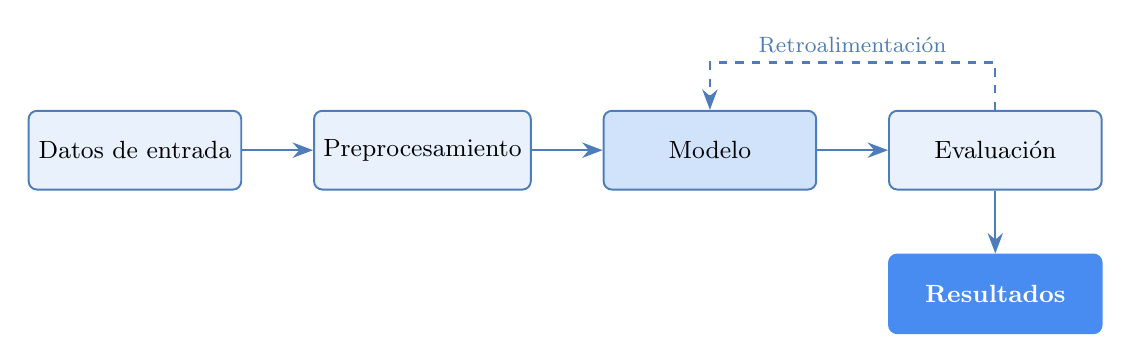
\begin{tikzpicture}[font=\small, node distance=9mm,
  caja/.style={draw=oscuro, line width=0.7pt, rounded corners=3pt, fill=claro!18,
               minimum width=27mm, minimum height=10mm, align=center},
  flecha/.style={-{Stealth[length=2.6mm]}, line width=0.8pt, draw=oscuro}]
  \node[caja] (a) {Datos de entrada};
  \node[caja, right=of a] (b) {Preprocesamiento};
  \node[caja, right=of b, fill=azul!25] (c) {Modelo};
  \node[caja, right=of c] (d) {Evaluación};
  \node[caja, below=8mm of d, fill=azul, text=white, draw=azul] (e) {\textbf{Resultados}};
  \draw[flecha] (a) -- (b); \draw[flecha] (b) -- (c); \draw[flecha] (c) -- (d); \draw[flecha] (d) -- (e);
  \draw[flecha, dashed] (d.north) -- ++(0,6mm) -| node[pos=0.25, above, font=\footnotesize, text=oscuro] {Retroalimentación} (c.north);
\end{tikzpicture}
\end{document}
